\documentclass{report}
\usepackage[utf8]{inputenc}
\usepackage[T1]{fontenc}
\usepackage[brazil]{babel}
\usepackage{graphicx}
\usepackage{amsfonts}
\usepackage{amssymb}
\usepackage{amsmath}
\usepackage{multicol}
\usepackage{ifthen}
\newboolean{firstanswerofthechapter}  
\usepackage{xcolor}
\colorlet{lightcyan}{cyan!40!white}
\usepackage{chngcntr}
\usepackage{stackengine}
\usepackage{tasks}
\usepackage{multirow}
\usepackage{float}
\newlength{\longestlabel}
\settowidth{\longestlabel}{\bfseries viii.}
%\settasks{counter-format={tsk[r].}, label-format={\bfseries}, label-width=\longestlabel,
    %item-indent=0pt, label-offset=2pt, column-sep={10pt}}
		
\setcounter{secnumdepth}{0} \setlength{\topmargin}{0cm}
\setlength{\headsep}{-0.3cm} \setlength{\textwidth}{17.5cm}
\setlength{\textheight}{23cm} \setlength{\oddsidemargin}{-0.8cm}
\setlength{\evensidemargin}{0cm} \setlength{\footskip}{-1.5cm}

\newcommand{\ad}{{\rm ad}}               %  adjunto
\newcommand{\tr}{{\rm tr}\,}             %  trace
\renewcommand{\dim}{{\rm dim}}           %  dimension
\newcommand{\real}{I\!\!R}               %  real numbers
\renewcommand{\zeta}{Z\! \! \! Z}        %  integer numbers
\newcommand{\ene}{I\! \! N}              %  natural numbers
\newcommand{\rac}{I\! \! \! Q}           %  rational numbers
\newcommand{\com}{\mathbb{C}}            %  complex numbers
\newcommand{\id}{{\rm Id}}               %  aplicaci\'on identidad
\newcommand{\Id}{{\rm Id}}               %  aplicaci\'on identidad
\newcommand{\di}{{\rm dim}}              %  dimensi\'on
\newcommand{\ce}{[\! [}                  %  claudator formes esquerra
\newcommand{\cd}{]\! ]}                  %  claudator formes dreta
\newcommand{\enmor}{{\rm End}\,}         %  Endomorfismes graduats
\newcommand{\Diff}{{\rm Diff}}           %  Op Difer graduats
\newcommand{\Hom}{{\rm Hom}\,}           %  Homomorfismes graduats
\newcommand{\Aut}{{\rm Aut}}             %  Automorfismes graduats

		
\usepackage[lastexercise,answerdelayed]{exercise}
%\counterwithin{Exercise}{chapter}
%\counterwithin{Answer}{chapter}
%\renewcounter{Exercise}[chapter]
%\newcommand{\QuestionNB}{\bfseries\arabic{Question}.\ }
%\renewcommand{\ExerciseName}{Exercício}
%\renewcommand{\ExerciseHeader}{\noindent\def\stackalignment{l}% code from https://tex.stackexchange.com/a/195118/101651
    %\stackunder[0pt]{\colorbox{cyan}{\textcolor{white}{\textbf{\LARGE\ExerciseHeaderNB\;\large\ExerciseName}}}}{\textcolor{lightcyan}{\rule{\linewidth}{2pt}}}\medskip}
\renewcommand{\ExerciseName}{Exercícios}
\renewcommand{\ExerciseHeader}{\noindent\def\stackalignment{l}% code from https://tex.stackexchange.com/a/195118/101651
    \stackunder[0pt]{\colorbox{cyan}{\textcolor{white}{\textbf{\large\ExerciseName}}}}{\textcolor{lightcyan}{\rule{\linewidth}{2pt}}}\medskip}
%\renewcommand{\AnswerName}{Exercises}
%\renewcommand{\AnswerHeader}{\ifthenelse{\boolean{firstanswerofthechapter}}%
    %{\bigskip\noindent\textcolor{cyan}{\textbf{CHAPTER \thechapter}}\newline\newline%
        %\noindent\bfseries\emph{\textcolor{cyan}{\AnswerName\ \ExerciseHeaderNB, page %
                %\pageref{\AnswerRef}}}\smallskip}
    %{\noindent\bfseries\emph{\textcolor{cyan}{\AnswerName\ \ExerciseHeaderNB, page \pageref{\AnswerRef}}}\smallskip}}
%\setlength{\QuestionIndent}{16pt}

\begin{document}

\vspace*{-2cm}

\begin{center}
\begin{minipage}[s]{2cm}
\hspace{-1.3cm}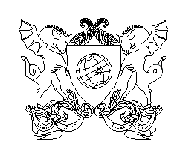
\includegraphics[scale=1.0]{/home/fsbmat/Documentos/GitHub/maf335.github.io/Brasao_UFV/brasaoufv.eps}
\end{minipage}
\begin{minipage}[s]{13cm}
{\begin{center} {\sc \Large Universidade Federal de Vi\c{c}osa}\\
{\sc \large Instituto de Ci\^encias Exatas e Tecnológicas}\\
{\sc \large Campus UFV - Florestal}\\
\end{center}}
\end{minipage}\begin{minipage}[s]{2 cm}
%\includegraphics[width=2 cm]{logoimecc.eps}
\end{minipage}
\end{center}

\vspace{-0.3cm}

%\hline \hline \noindent

%%%%%%%%%%%%%%%%%%%%%%%%%%%%%%%%%%%%%%%%%%%%%%%%%%%%%%%%%%%%%%%%%%%%%%%%%%%

\medskip

\begin{center}

\underline{\underline{{\large{\sc Álgebra Linear A - Gabarito da Lista 1}}}}

\bigskip

{\large {\bf Prof. Fernando Bastos}}
%\bigskip
%
%%{\sc Data: $19/06/2018$}
\end{center}


\begin{enumerate}

%%%%%%%%%%%%%%%%%%%%%%%%%%%%%%%%%%%%%%%%%%%%%%%%%%%%%%%%%%%%%%%%
%Exercicio 1
%%%%%%%%%%%%%%%%%%%%%%%%%%%%%%%%%%%%%%%%%%%%%%%%%%%%%%%%%%%%%%%%

\item $(a)$ $AE$ tem ordem $4 \times 5$, mas não é possível somar
com $B^T_{5 \times 4}$ pois têm ordens distintas;

$(b)$ não é possível somar $D^T_{5 \times 2}$ e $B_{4 \times 5}$
pois têm ordens distintas;

$(c)$ $\Big(A_{4 \times 3} \cdot C_{3 \times 5}\Big)_{4 \times 5}
+B_{4 \times 5}$ tem ordem $4 \times 5$;

$(d)$ não é possível mutliplicar $C$ por $B$, pois o número de
colunas de $C$ é igual $5$ que é diferente do número de colunas de
$B$, que é igual a $4$.

%%%%%%%%%%%%%%%%%%%%%%%%%%%%%%%%%%%%%%%%%%%%%%%%%%%%%%%%%%%%%%%%
%Exercicio 2
%%%%%%%%%%%%%%%%%%%%%%%%%%%%%%%%%%%%%%%%%%%%%%%%%%%%%%%%%%%%%%%%

\item $A$ tem ordem $5 \times 6$; \hspace{0.5cm} $B$ tem ordem $3
\times 6$; \hspace{0.5cm} $C$ tem ordem $3 \times 4$;
\hspace{0.5cm}

$D$ tem ordem $4 \times 3$ \hspace{0.5cm} e \hspace{0.5cm} $E$ tem
ordem $3 \times 5$.

%%%%%%%%%%%%%%%%%%%%%%%%%%%%%%%%%%%%%%%%%%%%%%%%%%%%%%%%%%%%%%%%
%Exercicio 3
%%%%%%%%%%%%%%%%%%%%%%%%%%%%%%%%%%%%%%%%%%%%%%%%%%%%%%%%%%%%%%%%

\item $(a)$ $A$ tem ordem $4 \times 5$; \hspace{1cm} $(b)$
$a_{23}=11$, \hspace{0.3cm} $a_{35}=3$ \hspace{0.3cm} e
\hspace{0.3cm} $a_{43}=-4$.


%%%%%%%%%%%%%%%%%%%%%%%%%%%%%%%%%%%%%%%%%%%%%%%%%%%%%%%%%%%%%%%%
%Exercicio 4
%%%%%%%%%%%%%%%%%%%%%%%%%%%%%%%%%%%%%%%%%%%%%%%%%%%%%%%%%%%%%%%%

\item $A$ tem ordem $3 \times 2$; \hspace{0.5cm} $B$ tem ordem $2
\times 3$; \hspace{0.5cm} $C$ tem ordem $3 \times 2$;
\hspace{0.5cm}

$D$ tem ordem $2 \times 3$ \hspace{0.5cm} e \hspace{0.5cm} $E$ tem
ordem $3 \times 2$.

%%%%%%%%%%%%%%%%%%%%%%%%%%%%%%%%%%%%%%%%%%%%%%%%%%%%%%%%%%%%%%%%
%Exercicio 5
%%%%%%%%%%%%%%%%%%%%%%%%%%%%%%%%%%%%%%%%%%%%%%%%%%%%%%%%%%%%%%%%

\item $c_{32}=18$ \hspace{0.3cm} e \hspace{0.3cm} $d_{48}=23$.


%%%%%%%%%%%%%%%%%%%%%%%%%%%%%%%%%%%%%%%%%%%%%%%%%%%%%%%%%%%%%%%%
%Exercicio 6
%%%%%%%%%%%%%%%%%%%%%%%%%%%%%%%%%%%%%%%%%%%%%%%%%%%%%%%%%%%%%%%%

\item $A= \left[
\begin{array}{rrrr}
3 & -4 & -7 & -10 \\
-2 & 8 & -5 & -8 \\
-5 & -1 & 15 & -6 \\
-8 & -4 & 0 & 24
\end{array}
\right]$.
%%%%%%%%%%%%%%%%%%%%%%%%%%%%%%%%%%%%%%%%%%%%%%%%%%%%%%%%%%%%%%%%
%Exercicio 7
%%%%%%%%%%%%%%%%%%%%%%%%%%%%%%%%%%%%%%%%%%%%%%%%%%%%%%%%%%%%%%%%

\item $(a)$ $A^2 = I_2$; \hspace{1.5cm} $(b)$
$A^3=A$;\hspace{1.5cm} $(c)$ $A^{31}=A$; \hspace{1.5cm} $(d)$
$A^{42}=I_2$.

%%%%%%%%%%%%%%%%%%%%%%%%%%%%%%%%%%%%%%%%%%%%%%%%%%%%%%%%%%%%%%%%
%Exercicio 8
%%%%%%%%%%%%%%%%%%%%%%%%%%%%%%%%%%%%%%%%%%%%%%%%%%%%%%%%%%%%%%%%

\item $x = -1$ \hspace{0.5cm} e \hspace{0.5cm} $y =1$.

%%%%%%%%%%%%%%%%%%%%%%%%%%%%%%%%%%%%%%%%%%%%%%%%%%%%%%%%%%%%%%%%
%Exercicio 9
%%%%%%%%%%%%%%%%%%%%%%%%%%%%%%%%%%%%%%%%%%%%%%%%%%%%%%%%%%%%%%%%

\item $(a)$ $x =4$, \hspace{1cm}  $(b)$ $x =12$ \ \ $y =-8$ \ \ $z
=-4$,

$(c)$ $x= 2$, \ \ $ y=-7$ \ \ $ z = -2$ \ \ ou \ \ $x= -2$, \ \ $
y=-3$ \ \ $ z = 10$.
%%%%%%%%%%%%%%%%%%%%%%%%%%%%%%%%%%%%%%%%%%%%%%%%%%%%%%%%%%%%%%%%
%Exercicio 10
%%%%%%%%%%%%%%%%%%%%%%%%%%%%%%%%%%%%%%%%%%%%%%%%%%%%%%%%%%%%%%%%

\item $(a)$ $4E-2D = \left[
\begin{array}{rrr}
22 & - & 8 \\
-2 & 4 & 6 \\
10 & 0 & 4
\end{array}
\right]$; \hspace{2cm} $(b)$ $2A^{T}+C=\left[
\begin{array}{rrr}
7 & 2 & 4 \\
3 & 5 & 7
\end{array}
\right]$;

$(c)$ $\left( 2E^{T}-3D^{T}\right) ^{T}=\left[
\begin{array}{rrr}
9 & -13 & 0 \\
1 & 2 & 1 \\
-1 & -4 & -6
\end{array}
\right]$; \hspace{1.5cm} $(d)$ $\left( BA^{T}-2C\right)
^{T}=\left[
\begin{array}{rr}
10 & -6 \\
-14 & 2 \\
-6 & -8
\end{array}
\right]$;

$(e)$ $\left(-AC\right)^{T}+5D^{T}=\left[
\begin{array}{rrr}
8  &  0 & 9 \\
37 & -2 & 15 \\
16 & 13 & 27
\end{array}
\right];$

$(f)$ $B^{T}\left( CC^{T}-A^{T}A\right) = \left[
\begin{array}{rr}
40 & 72 \\
26 & 42
\end{array}
\right];$ \ \ 

$(g)$ $0_{3 \times 3}$.

%%%%%%%%%%%%%%%%%%%%%%%%%%%%%%%%%%%%%%%%%%%%%%%%%%%%%%%%%%%%%%%%
%Exercicio 11
%%%%%%%%%%%%%%%%%%%%%%%%%%%%%%%%%%%%%%%%%%%%%%%%%%%%%%%%%%%%%%%%

\item $(a)$ $\left[
\begin{array}{rr}
1 & 1 \\
1 & 1
\end{array}
\right];$

$(b)$ Dada $B=\left[
\begin{array}{cc}
a & b \\
c & d
\end{array}
\right] $, então $B^2 =A$ se, e somente se, $\left[
\begin{array}{cc}
a ^2 + bc & ab+bd \\
ac+dc & bc + d^2
\end{array}
\right]  =\left[
\begin{array}{cc}
5 & 0 \\
0 & 9
\end{array}
\right] \Leftrightarrow \left\{
\begin{array}{c}
a ^2 + bc = 5 \\
b \ (a+d) =0 \\
c \ (a+d) =0 \\
bc + d^2 =9
\end{array}\right.$ e as soluções deste sistema são $a = \pm\sqrt{5}$, $b =c=0$ e $d = \pm\sqrt{9}$.

Logo, as raízes de $A$ são $\left[
\begin{array}{cc}
\sqrt{5} & 0 \\
0 & \sqrt{9}
\end{array}
\right]$, \ \ $\left[
\begin{array}{cc}
\sqrt{5} & 0 \\
0 & -\sqrt{9}
\end{array}
\right]$, \ \ $\left[
\begin{array}{cc}
-\sqrt{5} & 0 \\
0 & \sqrt{9}
\end{array}
\right]$, \ \ e \ \ $\left[
\begin{array}{cc}
-\sqrt{5} & 0 \\
0 & -\sqrt{9}
\end{array}
\right]$.

$(c)$ Não, o sistema pode não ter solução


%%%%%%%%%%%%%%%%%%%%%%%%%%%%%%%%%%%%%%%%%%%%%%%%%%%%%%%%%%%%%%%%
%Exercicio 12
%%%%%%%%%%%%%%%%%%%%%%%%%%%%%%%%%%%%%%%%%%%%%%%%%%%%%%%%%%%%%%%%

\item $(a)$ $(A\pm B)^2 = (A\pm B) \cdot (A\pm B)= A^2 \pm AB \pm
BA +B^2=A^2 \pm 2AB+B^2; $

$(b)$ $(A-B)(A+B) = = A^2 +AB -BA- B^2=A^2 - B^2;$

$(c)$ $(A-B)(A^2 +AB+B^2)  = A^3 +A^2B +AB^2-BA^2-BAB-B^3$

$\hspace{5.3cm}= A^3 +A(AB) +(AB)B-(BA)A-(BA)B-B^3$

$\hspace{5.3cm}=A^3 +A(BA) +(AB)B-(AB)A-(AB)B-B^3= A^3 - B^3$.

%%%%%%%%%%%%%%%%%%%%%%%%%%%%%%%%%%%%%%%%%%%%%%%%%%%%%%%%%%%%%%%%
%Exercicio 13
%%%%%%%%%%%%%%%%%%%%%%%%%%%%%%%%%%%%%%%%%%%%%%%%%%%%%%%%%%%%%%%%

\item $(a)$ $\Big(A\cdot A^T\Big)^T=(A^T)^T\cdot A^T=A \cdot A^T$;

\hspace{0.7cm}
$\Big(\frac{1}{2}(A+A^T)\Big)^T=\frac{1}{2}\Big(A^T+ (A^T)^T\Big)=
A +A^T.$

$(b)$
$\Big(\frac{1}{2}(A-A^T)\Big)^T=\frac{1}{2}\Big((A^T-(A^T)^T\Big)=
\frac{1}{2}\Big(A^T- A\Big)= -\frac{1}{2}(A-A^T).$

$(c)$ $A =
\frac{1}{2}\Big(A+A+A^T-A^T\Big)=\frac{1}{2}(A+A^T)+\frac{1}{2}(A-A^T)$.

%%%%%%%%%%%%%%%%%%%%%%%%%%%%%%%%%%%%%%%%%%%%%%%%%%%%%%%%%%%%%%%%
%Exercicio 14
%%%%%%%%%%%%%%%%%%%%%%%%%%%%%%%%%%%%%%%%%%%%%%%%%%%%%%%%%%%%%%%%

\item $(a)$ $\det A = \pm 1$

$(b)$ $A$ é anti-simétrica $\Leftrightarrow A=\left[
\begin{array}{rr}
0 & b \\
-b & 0
\end{array}
\right]$.

Por outro lado $A$ é ortogonal $\Leftrightarrow A \cdot A^T
=\left[
\begin{array}{rr}
0 & b \\
-b & 0
\end{array}
\right] \cdot \left[
\begin{array}{rr}
0 & -b \\
b & 0
\end{array}
\right]= \left[
\begin{array}{rr}
1 & 0 \\
0 & 1
\end{array}
\right]$, ou seja, $\Leftrightarrow b^2=1$.

Logo, as únicas matrizes quadradas de ordem $2$ que são
simultaneamente anti-simétricas e ortogonais são $\left[
\begin{array}{rr}
0 & -1 \\
1 & 0
\end{array}
\right]$ e $\left[
\begin{array}{rr}
0 & 1 \\
-1 & 0
\end{array}
\right]$.

%%%%%%%%%%%%%%%%%%%%%%%%%%%%%%%%%%%%%%%%%%%%%%%%%%%%%%%%%%%%%%%%
%Exercicio 15
%%%%%%%%%%%%%%%%%%%%%%%%%%%%%%%%%%%%%%%%%%%%%%%%%%%%%%%%%%%%%%%%

\item $m = \pm 1$.

%%%%%%%%%%%%%%%%%%%%%%%%%%%%%%%%%%%%%%%%%%%%%%%%%%%%%%%%%%%%%%%%
%Exercicio 16
%%%%%%%%%%%%%%%%%%%%%%%%%%%%%%%%%%%%%%%%%%%%%%%%%%%%%%%%%%%%%%%%

\item $A$ é ortogonal; \ \ $B$ não é ortogonal; \ \ $C$ é
ortogonal \ \ e \ \ $D$ é ortogonal.


%%%%%%%%%%%%%%%%%%%%%%%%%%%%%%%%%%%%%%%%%%%%%%%%%%%%%%%%%%%%%%%%
%Exercicio 17
%%%%%%%%%%%%%%%%%%%%%%%%%%%%%%%%%%%%%%%%%%%%%%%%%%%%%%%%%%%%%%%%

\item \label{1lista17} Dado $\alpha$ número real considere a
matriz $T_\alpha=\left[
\begin{array}{rr}
\cos \alpha & -\sin \alpha \\
\sin \alpha & \cos \alpha
\end{array}
\right]$.

$(a)$ $T_\alpha \cdot T_\beta=\left[
\begin{array}{rr}
\cos \alpha & -\sin \alpha \\
\sin \alpha & \cos \alpha
\end{array}
\right] \cdot \left[
\begin{array}{rr}
\cos \alpha & -\sin \alpha \\
\sin \alpha & \cos \alpha
\end{array}
\right] $

$\hspace{2cm}= \left[
\begin{array}{rrr}
\cos \alpha \cos \beta - \sin\alpha \sin \beta & &
-\cos \alpha \sin \beta -\sin \alpha \cos \beta \\
\sin \alpha  \cos \beta +\cos \alpha \sin \beta &  & - \sin \alpha
\sin \beta + \cos \alpha \cos \beta
\end{array}
\right] $

$\hspace{2cm}= \left[
\begin{array}{rr}
\cos (\alpha+\beta) & -\sin (\alpha+\beta) \\
\sin (\alpha+\beta) & \cos (\alpha+\beta)
\end{array}
\right] = T_{\alpha +\beta}$.

$(b)$ $T_{-\alpha}\left[
\begin{array}{rr}
\cos (-\alpha) & - \sin (-\alpha) \\
\sin (-\alpha) & \cos (-\alpha)
\end{array}
\right] = \left[
\begin{array}{rr}
\cos \alpha & - \ (-\sin \alpha) \\
-\sin \alpha & \cos \alpha
\end{array}
\right]=\left[
\begin{array}{rr}
\cos \alpha & \sin \alpha \\
-\sin \alpha & \cos \alpha
\end{array}
\right]$.

$(c)$ $T_\alpha \cdot T_\alpha^T=\left[
\begin{array}{rr}
\cos \alpha & -\sin \alpha \\
\sin \alpha & \cos \alpha
\end{array}
\right] \cdot \left[
\begin{array}{rr}
\cos \alpha & -\sin \alpha \\
\sin \alpha & \cos \alpha
\end{array}
\right]^T= \left[
\begin{array}{rr}
\cos \alpha & -\sin \alpha \\
\sin \alpha & \cos \alpha
\end{array}
\right] \cdot \left[
\begin{array}{rr}
\cos \alpha & \sin \alpha \\
-\sin \alpha & \cos \alpha
\end{array}
\right]$

$\hspace{1.8cm}=\left[
\begin{array}{ccc}
\cos^2 \alpha  + \sin^2 \alpha & & \cos \alpha \sin \alpha -\sin \alpha \cos \alpha \\
\sin \alpha \cos \alpha - \cos \alpha \sin \alpha & & \sin^2
\alpha + \cos^2 \alpha
\end{array}
\right]= \left[
\begin{array}{rr}
1 & 0 \\
0 & 1
\end{array}
\right]=I_2.$


%%%%%%%%%%%%%%%%%%%%%%%%%%%%%%%%%%%%%%%%%%%%%%%%%%%%%%%%%%%%%%%%
%Exercicio 18
%%%%%%%%%%%%%%%%%%%%%%%%%%%%%%%%%%%%%%%%%%%%%%%%%%%%%%%%%%%%%%%%

\item De fato, se $AB-BA=I$, então $\textrm{tr}(AB-BA) =
\textrm{tr}(I)=n$, mas por outro lado temos:

$\textrm{tr}(AB-BA) \stackrel{(a)}{=} \textrm{tr}(AB) +
\textrm{tr}(-BA)\stackrel{(b)}{=} \textrm{tr}(AB) -
\textrm{tr}(BA)\stackrel{(d)}{=} \textrm{tr}(AB) -
\textrm{tr}(AB)=0$ uma contradição.

Logo, não existe tal matriz.


%%%%%%%%%%%%%%%%%%%%%%%%%%%%%%%%%%%%%%%%%%%%%%%%%%%%%%%%%%%%%%%%

%%%%%%%%%%%%%%%%%%%%%%%%%%%%%%%%%%%%%%%%%%%%%%%%%%%%%%%%%%%%%%%%
%Exercicio 19
%%%%%%%%%%%%%%%%%%%%%%%%%%%%%%%%%%%%%%%%%%%%%%%%%%%%%%%%%%%%%%%%

\item Os traços de $AA^{T}$ e $A^{T}A$ estão definidos, pois são
matrizes quadradas de ordem $m \times m$ e $n \times n$,
respectivamente.

Agora considere $C=AA^{T}_{m \times m}$, então
$c_{ii}=\sum_{k=1}^{n} a^2_{ik}$, logo $$tr \ (AA^{T})=
\sum_{k=1}^{n} a^2_{1k} + \sum_{k=1}^{n} a^2_{2k}+ \ldots +
\sum_{k=1}^{n} a^2_{mk}.$$

Por outro lado, $D=A^{T}A$ é tal que $d_{ii}=\sum_{k=1}^{m}
a^2_{ki}$, logo $$tr \ (A^{T}A)= \sum_{k=1}^{m} a^2_{k1} +
\sum_{k=1}^{m} a^2_{k2}+ \ldots + \sum_{k=1}^{m} a^2_{kn}.$$

Logo, $tr \ (AA^{T})=tr \ (A^{T}A)$.

%%%%%%%%%%%%%%%%%%%%%%%%%%%%%%%%%%%%%%%%%%%%%%%%%%%%%%%%%%%%%%%%
%Exercicio 20
%%%%%%%%%%%%%%%%%%%%%%%%%%%%%%%%%%%%%%%%%%%%%%%%%%%%%%%%%%%%%%%%

\item $A^T=(A^{T}A)^T=A^T (A^T)^T=A^TA=A$, portanto $A$ é
simétrica.

Logo, $A=A^TA=AA=A^2$.


%%%%%%%%%%%%%%%%%%%%%%%%%%%%%%%%%%%%%%%%%%%%%%%%%%%%%%%%%%%%%%%%
%Exercicio 21
%%%%%%%%%%%%%%%%%%%%%%%%%%%%%%%%%%%%%%%%%%%%%%%%%%%%%%%%%%%%%%%%

\item Se $A=\left[
\begin{array}{cccc}
a_{11} & a_{12} & \cdots  & a_{1n} \\
a_{21} & a_{22} & \cdots  & a_{2n} \\
\vdots  & \vdots  & \ddots  & \vdots  \\
a_{n1} & a_{n2} & \cdots  & a_{nn}
\end{array}
\right],$ e $D=\left[
\begin{array}{cccc}
d_{11} & 0 & \cdots  & 0 \\
0 & d_{22} & \cdots  & 0 \\
\vdots  & \vdots  & \ddots  & \vdots  \\
0 & 0 & \cdots  & d_{nn}
\end{array}
\right],$ então $$A \cdot D =I_n \Leftrightarrow= \left[
\begin{array}{cccc}
a_{11} d_{11}& a_{12}d_{11} & \cdots  & a_{1n} d_{11}\\
a_{21} d_{22}& a_{22}d_{22} & \cdots  & a_{2n}d_{22} \\
\vdots  & \vdots  & \ddots  & \vdots  \\
a_{n1} d_{nn}& a_{n2}d_{nn} & \cdots  & a_{nn}d_{nn}
\end{array}
\right]= \left[
\begin{array}{cccc}
1 & 0 & \cdots  & 0 \\
0 & 1 & \cdots  & 0 \\
\vdots  & \vdots  & \ddots  & \vdots  \\
0 & 0 & \cdots  1
\end{array}
\right],$$ ou seja, se, e somente se, $a_{ij} = 0$ se $i \ne j$ e
$a_{ii} = (d_{ii})^{-1}$, ou seja, se, e somente se, $A$ é a
matriz diagonal inversa de $D$.


%%%%%%%%%%%%%%%%%%%%%%%%%%%%%%%%%%%%%%%%%%%%%%%%%%%%%%%%%%%%%%%%
%Exercicio 22
%%%%%%%%%%%%%%%%%%%%%%%%%%%%%%%%%%%%%%%%%%%%%%%%%%%%%%%%%%%%%%%%

%\item \label{1lista22}  Encontre uma matriz triangular superior
%tal que $ A^{3}=\left[
%\begin{array}{cc}
%1 & 30 \\
%0 & -8
%\end{array}
%\right].
%$

%%%%%%%%%%%%%%%%%%%%%%%%%%%%%%%%%%%%%%%%%%%%%%%%%%%%%%%%%%%%%%%%
%Exercicio 22
%%%%%%%%%%%%%%%%%%%%%%%%%%%%%%%%%%%%%%%%%%%%%%%%%%%%%%%%%%%%%%%%

\item Como $a_{11},a_{22},\dots,a_{nn}\neq 0$, então $\det A =
a_{11}a_{22}...a_{nn}\neq 0$,  logo existe $A^{-1}$ e mais
$$A^{-1}=\left[
\begin{array}{cccc}
\frac{1}{a_{11}} & 0 & \cdots  & 0 \\
0 & \frac{1}{a_{22}} & \cdots  & 0 \\
\vdots  & \vdots  & \ddots  & \vdots  \\
0 & 0 & \cdots  & \frac{1}{a_{nn}}
\end{array}
\right].$$

%%%%%%%%%%%%%%%%%%%%%%%%%%%%%%%%%%%%%%%%%%%%%%%%%%%%%%%%%%%%%%%%

%\item Considere a matriz
%$$
%A=\left[
%\begin{array}{cc}
%a & b \\
%c & d
%\end{array}
%\right],$$ onde $ab-cd\neq 0$. Prove que $A$ é invertível. (Dica:
%use sua intuição para inferir um candidato à inversa de $A$).


%%%%%%%%%%%%%%%%%%%%%%%%%%%%%%%%%%%%%%%%%%%%%%%%%%%%%%%%%%%%%%%%
%\item Use o exercício \ref{1lista19} para encontrar a inversa de
%$$
%\left[
%\begin{array}{rr}
%\cos \theta  & \func{sen}\theta  \\
%-\func{sen}\theta  & \cos \theta
%\end{array}
%\right].$$

%%%%%%%%%%%%%%%%%%%%%%%%%%%%%%%%%%%%%%%%%%%%%%%%%%%%%%%%%%%%%%%%
%Exercicio 23
%%%%%%%%%%%%%%%%%%%%%%%%%%%%%%%%%%%%%%%%%%%%%%%%%%%%%%%%%%%%%%%%

\item $AB=AC \Leftrightarrow A^{-1}(AB)=A^{-1}(AC)\Leftrightarrow
(A^{-1}A)B=(A^{-1}A)C\Leftrightarrow I \cdot B = I \cdot C
\Leftrightarrow B=C.$


%%%%%%%%%%%%%%%%%%%%%%%%%%%%%%%%%%%%%%%%%%%%%%%%%%%%%%%%%%%%%%%%
%Exercicio 24
%%%%%%%%%%%%%%%%%%%%%%%%%%%%%%%%%%%%%%%%%%%%%%%%%%%%%%%%%%%%%%%%

\item Sim, basta ter $A$ e $B$ matrizes não quadradas, por exemplo
$$\left[
\begin{array}{rrr}
-1 & 1 & 0 \\
1 & 1 & -1
\end{array}
\right] \cdot  \left[
\begin{array}{rr}
1 & 1 \\
2 & 1 \\
3 & 1
\end{array}
\right] = \left[
\begin{array}{rr}
1 & 0 \\
0& 1
\end{array}
\right].$$


%%%%%%%%%%%%%%%%%%%%%%%%%%%%%%%%%%%%%%%%%%%%%%%%%%%%%%%%%%%%%%%%
%Exercicio 25
%%%%%%%%%%%%%%%%%%%%%%%%%%%%%%%%%%%%%%%%%%%%%%%%%%%%%%%%%%%%%%%%

\item  $( a)$ Primeiro observemos que como $ A^{2}-3A+I=0$, então
    $A(A-3I)=-I$, logo $A$ é inversível pois,
    $\det A \det(A-3I)=\det(A(A-3I))=\det(-I)=(-1)^n \ne 0.$

Agora, $A^{-1}(A(A-3I))=A^{-1}(-I) \Leftrightarrow A- 3I =
-A^{-1},$ ou seja, $A^{-1} = 3I - A$.

$(b)$ Basta mostrar que $(I-A)(A + A^2 + \ldots +A^n) = I$ e que
$(A + A^2 + \ldots +A^n)(I-A) = I$.

Mas, $(I-A)(A + A^2 + \ldots +A^n) = A + A^2 + \ldots +A^n - A -
A^2 - \ldots -A^n-A^{n+1} =I-A^{n+1}=I.$

A outra igualdade se mostra de maneira análoga.

%%%%%%%%%%%%%%%%%%%%%%%%%%%%%%%%%%%%%%%%%%%%%%%%%%%%%%%%%%%%%%%%
%Exercicio 26
%%%%%%%%%%%%%%%%%%%%%%%%%%%%%%%%%%%%%%%%%%%%%%%%%%%%%%%%%%%%%%%%

\item  $(a)$ $(F)$; \ \ $(b)$ $(V)$; \ \ $(c)$ $(V)$; \ \ $(V)$
$(F)$;

$(e)$ $(F)$; \ \ $(f)$ $(V)$; \ \ $(g)$ $(V)$; \ \ $(h)$ $(F)$; \
\ $(i)$ $(V)$.


%Supondo que $A$ e $B$ são matrizes quadradas de ordem $n$
%inversíveis, prove as seguintes igualdades:

%\begin{enumerate}
%\item $(A^{-1} + B^{-1})^{-1} = A (A + B)^{-1} B.$

%\item $(I +AB)^{-1} A = A (I + BA)^{-1}$.

%\item $(A + BB^T)B = A^{-1} B (I +B^TA^{_1}B)^{-1}.$

%\end{enumerate}

%%%%%%%%%%%%%%%%%%%%%%%%%%%%%%%%%%%%%%%%%%%%%%%%%%%%%%%%%%%%%%%

%%%%%%%%%%%%%%%%%%%%%%%%%%%%%%%%%%%%%%%%%%%%%%%%%%%%%%%%%%%%%%%%
%Exercicio 27
%%%%%%%%%%%%%%%%%%%%%%%%%%%%%%%%%%%%%%%%%%%%%%%%%%%%%%%%%%%%%%%%

\item $(a)$ $\det P = 1024$ \ \ $(b)$ Logo, por $(a)$ $P$ é
inversível;  \ \ $(c)$ $\det B = -9$; \ \ $(d)$$Q$ é inversível.


%%%%%%%%%%%%%%%%%%%%%%%%%%%%%%%%%%%%%%%%%%%%%%%%%%%%%%%%%%%%%%%%
%Exercicio 28
%%%%%%%%%%%%%%%%%%%%%%%%%%%%%%%%%%%%%%%%%%%%%%%%%%%%%%%%%%%%%%%%

\item $\det A =-5$ .

%%%%%%%%%%%%%%%%%%%%%%%%%%%%%%%%%%%%%%%%%%%%%%%%%%%%%%%%%%%%%%%%
%Exercicio 29
%%%%%%%%%%%%%%%%%%%%%%%%%%%%%%%%%%%%%%%%%%%%%%%%%%%%%%%%%%%%%%%%

\item $(a)$ $\det(AB)=576$.

$(b)$ $A^{-1}= \left[
\begin{array}{rrrr}
1 & \frac{5}{2} & \frac{17}{8} & -\frac{31}{12} \\
& & & \\
0 & \frac{1}{2} & \frac{3}{8} & -\frac{5}{12} \\
& & & \\
0 & 0 & \frac{1}{4} & \frac{1}{6} \\
& & & \\
0 & 0 & 0 & \frac{1}{3}
\end{array}
\right];$ \ \ $(c)$ $B^{-1}= \left[
\begin{array}{rrrr}
-\frac{1}{3} & 0 & 0 & 0 \\
& & & \\
-\frac{1}{4} & -\frac{1}{4} & 0 & 0 \\
& & & \\
-\frac{7}{6} & -\frac{1}{2} & -1 & 0 \\
& & & \\
-\frac{25}{24} & -\frac{3}{8} & -\frac{1}{2} & -\frac{1}{2}
\end{array}
\right];$

$(d)$ $(AB)^{-1}= \left[
\begin{array}{rrrr}
-\frac{1}{3} & -\frac{5}{6} & -\frac{17}{24} & \frac{31}{36} \\
& & & \\
-\frac{1}{4} & -\frac{3}{3} & -\frac{5}{8} & \frac{3}{4} \\
& & & \\
-\frac{7}{6} & -\frac{19}{6} & -\frac{35}{12} & \frac{55}{18} \\
& & & \\
-\frac{25}{24} & -\frac{67}{24} & -\frac{119}{48} & \frac{187}{72}
\end{array}
\right];$ \ \  $(e)$ $\det C =16.$

%%%%%%%%%%%%%%%%%%%%%%%%%%%%%%%%%%%%%%%%%%%%%%%%%%%%%%%%%%%%%%%%
%Exercicio 30
%%%%%%%%%%%%%%%%%%%%%%%%%%%%%%%%%%%%%%%%%%%%%%%%%%%%%%%%%%%%%%%%

\item  $Q^3 +2 Q^2 =0 \Leftrightarrow Q^3 = -2Q^2$, como $\det Q
\ne 0$, a igualdade acima é equivalente a $Q =-2I$, portanto $\det
Q = (-2)^n$.


%%%%%%%%%%%%%%%%%%%%%%%%%%%%%%%%%%%%%%%%%%%%%%%%%%%%%%%%%%%%%%%%
%Exercicio 31
%%%%%%%%%%%%%%%%%%%%%%%%%%%%%%%%%%%%%%%%%%%%%%%%%%%%%%%%%%%%%%%%

\item $(a)$ $\det A = 58$ \ \ $(b)$ $\det A^T =\det A = 58$; \ \
$(c)$ $\det A^2 = (\det A)^2 = 58^2 = 3364$;

$(d)$ $A^{-1}= \frac{1}{\det A}= \frac{1}{58}$;  \ \ $(e)$ $\det(
-A) = (-1)^4 \det A = 58$;

$(f)$ $\det(3AA^T)=3^4\det A \det A^T = 3^4 58^2 = 272.484$.

%%%%%%%%%%%%%%%%%%%%%%%%%%%%%%%%%%%%%%%%%%%%%%%%%%%%%%%%%%%%%%%%
%Exercicio 32
%%%%%%%%%%%%%%%%%%%%%%%%%%%%%%%%%%%%%%%%%%%%%%%%%%%%%%%%%%%%%%%%

\item  Determine o polinômio $p(x)=\det (xI_3 -A) =
\det\left(x\left[
\begin{array}{rrr}
1 & 0 & 0 \\
0 & 1 & 0 \\
0 & 0 & 1
\end{array}
\right] - \left[
\begin{array}{rrr}
1 & 1 & -1 \\
1 & 0 & 1 \\
0 & 1 & 1
\end{array}
\right] \right)= \det \left[
\begin{array}{rrr}
x-1 & -1 & 1 \\
-1 & x & -1 \\
0 & -1 & x-1
\end{array}
\right] = x(x-1)^2+1-2(x-1)=x^3-2x^2-x+3.$

$(b)$  $p(A)= A^3 -2A^2 -A +3I = 0$.

$(c)$  $A^3 -2A^2 -A +3I = 0 \Leftrightarrow A(A^2 -2A - I) =
-3I,$ portanto $A^{-1} = \frac{1}{3} (I+2A -A^2)$.

%%%%%%%%%%%%%%%%%%%%%%%%%%%%%%%%%%%%%%%%%%%%%%%%%%%%%%%%%%%%%%%%
%Exercicio 33
%%%%%%%%%%%%%%%%%%%%%%%%%%%%%%%%%%%%%%%%%%%%%%%%%%%%%%%%%%%%%%%%

\item $(a)$ $-123$ \ \  $(b)$ $1 + a + b +c$ \ \ $(c)$ $-c^4 +c^3
-16 c^2 +8c -2$ \ \ $(d)$  $-5$ \  \  $(e)$ $-120$  \ \ $(f)$
$120.$


%%%%%%%%%%%%%%%%%%%%%%%%%%%%%%%%%%%%%%%%%%%%%%%%%%%%%%%%%%%%%%%%
%Exercicio 34
%%%%%%%%%%%%%%%%%%%%%%%%%%%%%%%%%%%%%%%%%%%%%%%%%%%%%%%%%%%%%%%%

\item $(a)$ $ \{ 0, -1, 1/2\};$ \ \  $(b)$ $ \{\frac{40}{11}\};$ \
\  $(c)$ $ \{\frac{3 +\sqrt{33}}{4}, \ \frac{3 -\sqrt{33}}{4}\}.$

%%%%%%%%%%%%%%%%%%%%%%%%%%%%%%%%%%%%%%%%%%%%%%%%%%%%%%%%%%%%%%%%
%Exercicio 22
%%%%%%%%%%%%%%%%%%%%%%%%%%%%%%%%%%%%%%%%%%%%%%%%%%%%%%%%%%%%%%%%

%\item \label{1lista22}  Seja $A=\left[
%\begin{array}{rrr}
%-2 & 2 & 3 \\
%-2 & 3 & 2 \\
%-4 & 2 & 5
%\end{array}
%\right] $. Determine $x$, número real,  tal que $\det ( xI-A) =0$.



%%%%%%%%%%%%%%%%%%%%%%%%%%%%%%%%%%%%%%%%%%%%%%%%%%%%%%%%%%%%%%%%
%Exercicio 35
%%%%%%%%%%%%%%%%%%%%%%%%%%%%%%%%%%%%%%%%%%%%%%%%%%%%%%%%%%%%%%%%

\item $\det A = a_{14} a_{23} a_{32} a_{41}$, generalizando temos
$$\det A = \prod_{i=1}^{n}a_{i, n-i+1}.$$


%%%%%%%%%%%%%%%%%%%%%%%%%%%%%%%%%%%%%%%%%%%%%%%%%%%%%%%%%%%%%%%%%%%%%%%%%%%%%%%%%%%%
%%%%%%%%%%%%%%%%%%%%%%%%%%%%%%%%%%%%%%%%%%%%%%%%%%%%%%%%%%%%%%%%
%Exercicio 36
%%%%%%%%%%%%%%%%%%%%%%%%%%%%%%%%%%%%%%%%%%%%%%%%%%%%%%%%%%%%%%%%

\item $(a)$ $B= PAP^{-1} \Leftrightarrow P^{-1}BP=
P^{-1}(PAP^{-1})P\Leftrightarrow P^{-1}BP= (P^{-1}P)A(P^{-1}P)=A.$

Logo, $A = P^{-1}B(P^{-1})^{-1}$, ou seja, $B$ é semelhante a $A$.

$(b)$ Suponhamos que $B= PAP^{-1}$ e $C= QBQ^{-1}$, então $$C=
Q(PAP^{-1})Q^{-1}=(QP)A(P^{-1}Q^{-1})=(QP)A(QP)^{-1},$$ portanto
$A$ é semelhante a $C$.

$(c)$ Suponhamos que $A$ é semelhante a $B$, então $B= PAP^{-1}$,
onde $P$ é matriz inversível. Logo, $$\det B = \det (PAP^{-1}) =
\det P \det A \det P^{-1} = \det P \det A \frac{1}{\det P}= \det
A.$$

%%%%%%%%%%%%%%%%%%%%%%%%%%%%%%%%%%%%%%%%%%%%%%%%%%%%%%%%%%%%%%%%%%%%%%%%%

%\item  Expresse
%$$\left|
%\begin{array}{rr}
%a_{1}+b_{1} & c_{1}+d_{1} \\
%a_{2}+b_{2} & c_{2}+d_{2}
%\end{array}
%\right|,$$
%como uma soma de determinantes cujas entradas não contém
%somas.


%%%%%%%%%%%%%%%%%%%%%%%%%%%%%%%%%%%%%%%%%%%%%%%%%%%%%%%%%%%%%%%%%%%%%%%%%%%%%%

%\item  Prove que uma matriz quadrada $A$ é invertível se,
%e somente se, $A^{T}A$ é invertível.

%%%%%%%%%%%%%%%%%%%%%%%%%%%%%%%%%%%%%%%%%%%%%%%%%%%%%%%%%%%%%%%%%%%%%%%%%%%%%

%%%%%%%%%%%%%%%%%%%%%%%%%%%%%%%%%%%%%%%%%%%%%%%%%%%%%%%%%%%%%%%%
%Exercicio 24
%%%%%%%%%%%%%%%%%%%%%%%%%%%%%%%%%%%%%%%%%%%%%%%%%%%%%%%%%%%%%%%%

%\item \label{1lista24}  Mostre que as matrizes
%$$ A=\left[
%\begin{array}{rr}
%a & b \\
%0 & c
%\end{array}
%\right] \  \textrm{ e } \  B=\left[
%\begin{array}{rr}
%d & e \\
%0 & f
%\end{array}
%\right],$$ comutam se, e somente se, $\left|
%\begin{array}{rr}
%b & a-c \\
%e & d-f
%\end{array}
%\right| =0$.




%%%%%%%%%%%%%%%%%%%%%%%%%%%%%%%%%%%%%%%%%%%%%%%%%%%%%%%%%%%%%%%%
%Exercicio 37
%%%%%%%%%%%%%%%%%%%%%%%%%%%%%%%%%%%%%%%%%%%%%%%%%%%%%%%%%%%%%%%%

\item $(a)$ $cof(A)=\left[
\begin{array}{rrr}
29 & -21 & 27 \\
-11 & 13 & 5 \\
-19 & -19 & 19
\end{array}
\right];$ como $\det A = 152 \ne 0$, então existe $A^{-1}$ e
$$A^{-1}=\left[
\begin{array}{rrr}
\frac{29}{152} & -\frac{11}{152} & -\frac{1}{8}\\
& & \\
-\frac{21}{152} & \frac{13}{152} & -\frac{1}{8} \\
& & \\
\frac{27}{152} & \frac{5}{152} & \frac{1}{8}
\end{array}
\right].$$

$(b)$ 
$
cof(A)=\left[
\begin{array}{rrr}
\cos \theta  & \sin\theta  & 0 \\
-\sin\theta  & \cos \theta  & 0 \\
0 & 0 & 1
\end{array}
\right];$ 

como $\det A = 1 \ne 0$, então existe $A^{-1}$ e
$$A^{-1}=\left[
\begin{array}{rrr}
\cos \theta  & -\sin\theta  & 0 \\
\sin\theta  & \cos \theta  & 0 \\
0 & 0 & 1
\end{array}
\right].$$

\bigskip

$(c)$ $cof(A)=\left[
\begin{array}{rrrr}
-2 & -1 & 5 & -2 \\
2 & 1 & -5 & 4 \\
0 & 0 & 2 & -2 \\
0 & 1 & -1 & 0
\end{array}
\right];$  como $\det A = 1 \ne 0$, então existe $A^{-1}$ e
$$A^{-1}=\left[
\begin{array}{rrrr}
-1 &  1& 0 & 0 \\
& & & \\
-\frac{1}{2} & \frac{1}{2} & 0 & \frac{1}{2} \\
& & &\\
\frac{5}{2} & -\frac{5}{2} & 1 & -\frac{1}{2} \\
& & &\\
-1 & 2 & -1 & 0
\end{array}
\right].$$

$(d)$ $cof(A)=\left[
\begin{array}{rrrr}
0 & 0 & 12 & 16 \\
0 & -72 & 60 & 128 \\
18 & 36 & -39 & -106 \\
0 & 0 & 0 & 24
\end{array}
\right];$ como $\det A = 72 \ne 0$, então existe $A^{-1}$ e
$$A^{-1}=\left[
\begin{array}{rrrr}
0 &  0& \frac{1}{4} & 0 \\
& & & \\
0 & -1 & \frac{1}{2} &  0 \\
& & & \\
\frac{1}{6} & \frac{5}{6} & -\frac{13}{24} & 0 \\
& & & \\
\frac{2}{9} & \frac{16}{9} & -\frac{53}{36} & \frac{1}{3}
\end{array}
\right].$$

%%%%%%%%%%%%%%%%%%%%%%%%%%%%%%%%%%%%%%%%%%%%%%%%%%%%%%%%%%%%%%%%%%%%%%%%

%\item Prove que se $A$ é invertível, então $\func{adj}A$ é invertível e
%$$( \func{adj}A) ^{-1}=\dfrac{1}{\det A}A=\func{adj}(
%A^{-1}).$$

%%%%%%%%%%%%%%%%%%%%%%%%%%%%%%%%%%%%%%%%%%%%%%%%%%%%%%%%%%%%%%%%%%%%%%%%

%\item  Mostre que se $A$ é uma matriz $n\times n$, então
%$\det ( \func{adj}A) =( \det A)^{n-1}$.

%%%%%%%%%%%%%%%%%%%%%%%%%%%%%%%%%%%%%%%%%%%%%%%%%%%%%%%%%%%%%%%%%%%%%%%%


%%%%%%%%%%%%%%%%%%%%%%%%%%%%%%%%%%%%%%%%%%%%%%%%%%%%%%%%%%%%%%%%
%Exercicio 38
%%%%%%%%%%%%%%%%%%%%%%%%%%%%%%%%%%%%%%%%%%%%%%%%%%%%%%%%%%%%%%%%

\item Basta observar que a linha $L_1$ é proporcional às linhas
$L_2$ e $L_3$, pois $L_1 = (a+b+c)L_3 -L_2.$

Logo, o determinate da matriz é nulo.



%%%%%%%%%%%%%%%%%%%%%%%%%%%%%%%%%%%%%%%%%%%%%%%%%%%%%%%%%%%%%%%%
%Exercicio 39
%%%%%%%%%%%%%%%%%%%%%%%%%%%%%%%%%%%%%%%%%%%%%%%%%%%%%%%%%%%%%%%%

\item $(a)$ $\det A=32 \ne 0$, logo existe $A^{-1}$ e
$A^{-1}=\left[
\begin{array}{rrr}
-\frac{1}{8} & \frac{3}{8} & -\frac{1}{8} \\
& & \\
-\frac{1}{4} & 0 & \frac{1}{4} \\
& & \\
\frac{1}{2} & -\frac{1}{4} & 0
\end{array}
\right].$

$(b)$ $\det A=14 \ne 0$, logo existe $A^{-1}$ e $A^{-1}=\left[
\begin{array}{rr}
\frac{2}{7} & \frac{1}{14} \\
& \\
 -\frac{1}{7} & \frac{3}{14}
\end{array}
\right].$


$(c)$ $\det A=1 \ne 0$ logo existe $A^{-1}$ e $A^{-1}=\left[
\begin{array}{rrrr}
1 & 0 & 0 & 0 \\
-2 & 1 & 0 & 0 \\
1 & -2 & 1 & 0 \\
0 & 1 & -2 & 1
\end{array}
\right].$

$(d)$ $\det A=-459 \ne 0$ logo existe $A^{-1}$ e $A^{-1}=\left[
\begin{array}{rrr}
-\frac{5}{51} & -\frac{28}{51} & -\frac{2}{51} \\
& & \\
-\frac{2}{51} & \frac{16}{51} & \frac{1}{51} \\
& & \\
-\frac{2}{51} & -\frac{1}{51} & \frac{1}{51}
\end{array}
\right].$


%%%%%%%%%%%%%%%%%%%%%%%%%%%%%%%%%%%%%%%%%%%%%%%%%%%%%%%%%%%%%%%%
%Exercicio 40
%%%%%%%%%%%%%%%%%%%%%%%%%%%%%%%%%%%%%%%%%%%%%%%%%%%%%%%%%%%%%%%%

\item $\det B=1 \ne 0$ logo existe $B^{-1}$ e $$B^{-1}=\left[
\begin{array}{rrrrrr}
0 & 0 & -1 & 0 & 0 & 0 \\
0 & 0 & 0 & 0 & -1 & 0\\
0 & 0 & 0 & 0 & 0 & -1\\
1 & 0 & 0 & 0 & 0 & 0 \\
0 & 0 & 0 & 1 & 0 & 0 \\
0 & 1 & 0 & 0 & 0 & 0
\end{array}
\right].$$

%%%%%%%%%%%%%%%%%%%%%%%%%%%%%%%%%%%%%%%%%%%%%%%%%%%%%%%%%%%%%%%%
%Exercicio 41
%%%%%%%%%%%%%%%%%%%%%%%%%%%%%%%%%%%%%%%%%%%%%%%%%%%%%%%%%%%%%%%%

\item $(a)$ $(F)$; \ \ $(b)$ $(F)$; \ \ $(c)$ $(V)$; \ \ $(d)$
$(F)$;

$(e)$ $(F)$; \ \ $(f)$ $(F)$; \ \ $(g)$ $(V)$; \ \ $(h)$ $(V)$; \
\ $(i)$ $(V)$.

%%%%%%%%%%%%%%%%%%%%%%%%%%%%%%%%%%%%%%%%%%%%%%%%%%%%%%%%%%%%%%%%
%Exercicio 42
%%%%%%%%%%%%%%%%%%%%%%%%%%%%%%%%%%%%%%%%%%%%%%%%%%%%%%%%%%%%%%%%

\item $(a)$ Dia a Dia:$145.400$, \ \ Nossa Hora: $213.200$, \ \
Acontece: $164.850$ \ \ Urgente: $239.250$.

$(b)$ Dia a Dia:$232.640$, \ \ Nossa Hora: $341.120$, \ \
Acontece: $263.760$, \ \ Urgente: $382.800$.


%%%%%%%%%%%%%%%%%%%%%%%%%%%%%%%%%%%%%%%%%%%%%%%%%%%%%%%%%%%%%%%%
%Exercicio 43
%%%%%%%%%%%%%%%%%%%%%%%%%%%%%%%%%%%%%%%%%%%%%%%%%%%%%%%%%%%%%%%%

\item $(a)$ Tábuas: $19.000$, \ \ Tijolos: $450.000$, \ \ Telhas:
$375.000$, \ \ Tinta: $2.750$ litros, \ \ Mão de obra: $2.000$
dias.

$(b)$ A primeira coluna de $AB$ representa o custo dos materiais
para as $20$ construções de alvenaria, as $15$ construções de
madeira e as $30$ construções mistas, respectivamente; enquanto
que a segunda coluna representa o custo do transporte para as $20$
construções de alvenaria, as $15$ construções de madeira e as $30$
construções mistas, respectivamente.

%%%%%%%%%%%%%%%%%%%%%%%%%%%%%%%%%%%%%%%%%%%%%%%%%%%%%%%%%%%%%%%%
%Exercicio 44
%%%%%%%%%%%%%%%%%%%%%%%%%%%%%%%%%%%%%%%%%%%%%%%%%%%%%%%%%%%%%%%%

\item A quantidade necessária será: $780 g$ de fósforo, $555 g$ de
nitrato e $1.455 g$ de potássio. O preço totalda mistura será $
R\$154,50.$



%%%%%%%%%%%%%%%%%%%%%%%%%%%%%%%%%%%%%%%%%%%%%%%%%%%%%%%%%%%%%%%%
%Exercicio 45
%%%%%%%%%%%%%%%%%%%%%%%%%%%%%%%%%%%%%%%%%%%%%%%%%%%%%%%%%%%%%%%%

\item $A=\left[
\begin{array}{rrr}
1 & 3 & 1 \\
2 & 5 & 1 \\
1,5 & 4 & 1
\end{array}
\right]$,  $B=\left[
\begin{array}{rr}
2 & 1,5 \\
1 & 1,8 \\
0,5 & 0,6
\end{array}
\right]$ e $AB=\left[
\begin{array}{rr}
5,5 & 7,5 \\
9,5 & 12,6 \\
7,5 & 10,05
\end{array}
\right].$

O significado de $AB$ é o custo da produção de cada produto em
cada uma das duas cidades.


%%%%%%%%%%%%%%%%%%%%%%%%%%%%%%%%%%%%%%%%%%%%%%%%%%%%%%%%%%%%%%%%
%Exercicio 46
%%%%%%%%%%%%%%%%%%%%%%%%%%%%%%%%%%%%%%%%%%%%%%%%%%%%%%%%%%%%%%%%

\item $AB^T=\left[
\begin{array}{rrr}
71.000 & 47.000 & 110.000 \\
97.000 & 29.000 & 39.000 \\
114.000 & 65.500 & 176.000
\end{array}
\right].$

\end{enumerate}

\end{document}

\end{document}